%Este trabalho está licenciado sob a Licença Creative Commons Atribuição-CompartilhaIgual 4.0 Internacional. Para ver uma cópia desta licença, visite https://creativecommons.org/licenses/by-sa/4.0/ ou envie uma carta para Creative Commons, PO Box 1866, Mountain View, CA 94042, USA.

\section{Exercícios}

\begin{exer}
 (Sociesc - 2010) Considere um triângulo equilátero de lado $l$. Unindo-se os pontos médios dos seus lados obtemos 4 novos triângulos. O perímetro de qualquer um desses novos triângulos é igual a:

 \begin{multicols}{2}

 \begin{enumerate}[a)]
  \item $\frac{3l}{2}$
  \item $\frac{5l}{2}$
  \item $l$
  \item $3l$
 \end{enumerate}

 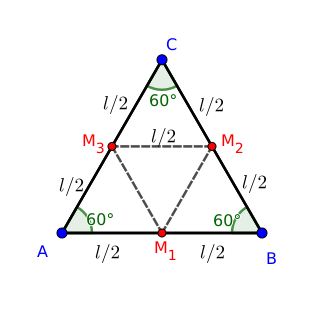
\includegraphics[width=5cm]{Capitulos/Figuras/tri_equi_exer1.pdf}

 \end{multicols}
 \end{exer}

  \begin{exer}
 (UDESC/Fepese - 2009) Seja $ABCD$ o paralelogramo abaixo, e seja $E$ um ponto no segmento $\overline{AD}$, conforme descrito na figura abaixo:

  \begin{center}
 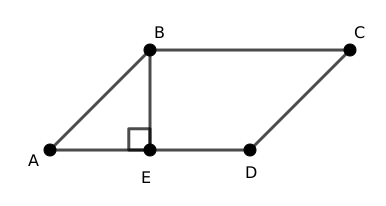
\includegraphics[width=4cm]{Capitulos/Figuras/udesc2009.pdf}
 \end{center}

  Sabendo que $\overline{AB} = 5$, $\overline{AE} = 3$ e $\overline{AD} = 8$, a área do paralelogramo $ABCD$ é:
  \begin{enumerate}[a)]
  \item 15
  \item 24
  \item 30
  \item 32
  \item 40
 \end{enumerate}
 \end{exer}

 \begin{exer}
 (UDESC/IBC - 2009) Em um cone eqüilátero, a área lateral mede $128 \pi cm^2$. O raio da base desse cone, em cm, é:
 \begin{enumerate}[a)]
  \item 6
  \item 7
  \item 8
  \item 9
  \item 10
 \end{enumerate}
 \end{exer}

 Gabarito: 1 a); 2 d).
